\section{ps5: DNA Alignment}\label{sec:ps5}

\subsection{Overview}\label{sec:ps5:overview} % A discussion of the assignment itself

This project computes the optimal sequence alignment for two DNA strings.
It aligns two DNA sequences using a least cost method.

\subsection{End Product}\label{sec:ps5:accomplish} % What I accomplished and images/results

Below is the output.
This aligns two DNA strings with the cost of the total alignment at the top with the cost of each alignment as the last column.

\begin{figure}[h]
\centering
\begin{minipage}[b]{0.4\textwidth}
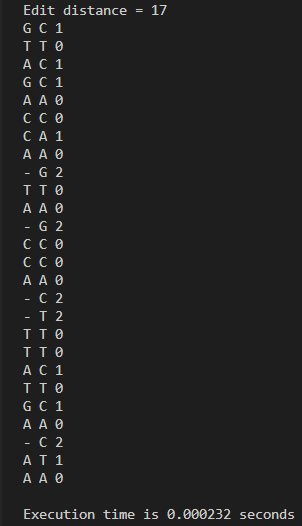
\includegraphics[width=\textwidth]{ps5-1_output}
\caption{"stx26" DNA Alignment}
\end{minipage}
\end{figure}

\subsection{What I Already Knew}\label{sec:ps5:knew} % What was known prior to the assignment

I knew how to create a matrix to store the cumulative penalties.

\subsection{Design Decisions and Implementations}\label{sec:ps5:decisions} % Important decisions or implementations I made

The project uses the Needleman-Wunsch of dynamic programming. 
It was implemented through the EDistance class, which takes two strings of length N and M, and creates an N x M matrix of integers.
To compute the value of each value in the matrix it was broken into sub-problems.
The final row and final column can be computed from the lengths of the given strings.
For filling everything else, we work backwards from the \[N\]\[M\] by filling it with the minimum of three values. 
These three values are the three possible cases: A letter of a string aligning with the same letter, a different letter, or a gap and finds the best comparison.
Once the matrix is filled, the penalty of alignment can be found at \[0\]\[0\].
The actual alignment can be traced backwards using a similar way we populated the matrix.

\subsection{What I Learned}\label{sec:ps5:learned} % What I learned because of the assignment

I learned what the Needleman-Wunsch dynamic programming method is and how it can be beneficial to reduce time complexity.

\subsection{Challenges}\label{sec:ps5:challenges} % Challenges along the way and any that went unresolved

There were no major challenge as the project guide layed ot a good foundation for writing the code.

\newpage
\subsection{Codebase}\label{sec:ps5:code} % Code: Makefile, .cpp main, .hpp main, .cpp support, .hpp support, .cpp tests

\bigskip
\title{\large Makefile:}
\lstinputlisting{../ps5/Makefile}
\bigskip
\title{\large main.cpp:}
\lstinputlisting{../ps5/main.cpp}
\bigskip
\title{\large Checkers.cpp:}
\lstinputlisting{../ps5/EDistance.cpp}
\bigskip
\title{\large Checkers.hpp:}
\lstinputlisting{../ps5/EDistance.hpp}

\newpage
